\documentclass[12pt]{article}

% Dependencies
\usepackage[left=1cm, right=1cm, top=.5cm, bottom=.5cm]{geometry}
\usepackage{xcolor}
\usepackage{graphicx}
\usepackage{calc}
\usepackage[T1]{fontenc}
\usepackage[utf8]{inputenc}
\usepackage{enumitem}
\usepackage{mdframed}
\usepackage{amssymb}
\usepackage{ifmtarg}
\usepackage{multicol}

% Mettrics
\setlength\parindent{0pt}
\setlength\fboxsep{0pt}

\newlength\cvPhotoWidth
\setlength\cvPhotoWidth{3cm}

\newlength\cvHspacePhotoTitle
\setlength\cvHspacePhotoTitle{.5cm}

\newlength\cvVspacePhotoTitle
\setlength\cvVspacePhotoTitle{.5cm}

\newlength\cvLeftWidth
\setlength\cvLeftWidth{0.5\textwidth}

\newlength\cvHspaceLeftRight
\setlength\cvHspaceLeftRight{.5cm}

\newlength\cvNameWidth
\setlength\cvNameWidth{10.5cm}

\newlength\cvAddressWidth
\setlength\cvAddressWidth{\textwidth-\cvPhotoWidth-\cvNameWidth-1cm}

\newlength\cvRightWidth
\setlength\cvRightWidth{\textwidth-\cvLeftWidth-\cvHspaceLeftRight-0.5cm}

\definecolor{lightgray}{HTML}{efefef}

\setlist[itemize]{noitemsep, topsep=0pt, leftmargin=15pt}
\renewcommand{\labelitemi}{{\tiny$\blacksquare$}}

\pagenumbering{gobble}

\newcommand\cvBullet{ $\blacksquare$ }

\newcommand\cvSection[1]{
    \begin{mdframed}[
        linewidth=.5pt,
        topline=false,
        leftline=false,
        rightline=false,
        linecolor=red!60!black,
        innermargin=0,
        outermargin=0
    ]
        \begin{Large}
            \textbf{#1}
        \end{Large}
    \end{mdframed}
}

\newcommand\cvItem[5]{
    \def\cvPlace{#4}
    \begin{mdframed}[
        linewidth=1.5pt,
        topline=false,
        bottomline=false,
        rightline=false,
        linecolor=red!60!black,
        innermargin=0,
        outermargin=0,
        backgroundcolor=lightgray
    ]
        \textit{#1}\\
        \begin{normalsize}
            \textbf{#2}
        \end{normalsize}\\
        \textcolor{red!60!black}{#3}
        \ifx\cvPlace\empty\else - #4 \fi
    \end{mdframed}
    #5
}

\begin{document}

    \begin{minipage}[t]{\textwidth}
        \begin{minipage}{\cvPhotoWidth}
            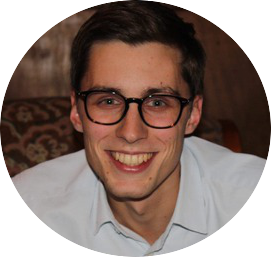
\includegraphics[width=\textwidth]{src/profile.png}
        \end{minipage}
        \hspace{\cvHspacePhotoTitle}
            \begin{minipage}[t]{\textwidth-\cvPhotoWidth-\cvHspacePhotoTitle}
            \begin{minipage}{\cvNameWidth}
            \begin{Huge}
                \textbf{Henri Lefebvre}
            \end{Huge}
            22 ans\\
            Cherche stage en optimisation/apprentissage automatique
            \end{minipage}
            \begin{minipage}{\cvAddressWidth}
                \begin{flushright}
                    33 Rue des Cronquelets, \\
                    Saint-Aubin, 62170 (FR)\\
                    \underline{henri.lefebvre@yahoo.com}\\
                    07 78 34 29 49\\
                    Permis B
                \end{flushright}
            \end{minipage}
        \end{minipage}
    \end{minipage}
    \begin{minipage}[t]{\textwidth}
        \vspace{\cvVspacePhotoTitle}
        \begin{minipage}[t]{\cvLeftWidth}
            \cvSection{Projets et réalisations}
            \cvItem{Février 2018 - Juin 2018}{Planificateur d'itinéraire multimodal}{Laboratoire Heudiasyc}{Compiègne}{
                \begin{itemize}
                    \item Exploitation de données \textit{Google Transit Format Specification} (GTFS) pour la génération du graphe
                    \item Algorithme de Dijkstra avec dépendence temporelle
                \end{itemize}
                \textit{Dijkstra, time dependent model, graphes}
            }
            \cvItem{Juin 2017}{Optimisation de la charge de wagons}{Université de Technologie de Compiègne}{}{
                \begin{itemize}
                    \item Utilisation du solveur XPress MP
                    \item Modélisation linéaire du problème
                \end{itemize}
                \textit{Multidimensional knapsack problem, XPress MP}
            }
            \cvItem{Avril 2017 - Juin 2017}{Intelligence artificielle pour jeu de plateau}{Université de Technologie de Compiègne}{}{
                \begin{itemize}
                    \item Programmation logique pour la création de l'IA
                    \item Joueur autonome pour le jeu Arimaa
                \end{itemize}
                \textit{Prolog, intelligence artificielle symbolique}
            }
            \cvSection{Expériences professionnelles}
            \cvItem{Septembre 2018 - Aout 2018}{Développeur backend sous AWS}{MoneyCup}{Paris}{
                \begin{itemize}
                    \item Développement du moteur d'investissement
                    \item Création du backend de l'application mobile
                    \item Implémentation d'une solution de e-signature
                    \item Gestion d'événements asynchrones/parrallèles
                \end{itemize}
                \textit{Finance, AWS, NoSQL, DynamoDB, node.js}
            }
            \cvItem{Février 2018}{Stagiaire - assistant contrôle qualité}{Valeo}{Étaples}{}
        \end{minipage}
        \hspace{\cvHspaceLeftRight}
        \begin{minipage}[t]{\cvRightWidth}
            \cvSection{Diplômes}
            \cvItem{2018 - 2019}{\textit{Laurea Magistrale en Informatica}}{Università degli studi di Genova}{Italie}{}
            \cvItem{2018 - 2019}{Master \textit{Apprentissage et optimisation}}{Université de Technologie de Compiègne}{}{}
            \cvItem{2014 - 2019}{Ingénieur Génie Informatique}{Université de Technologie de Compiègne}{}{
                \begin{itemize}
                    \item Filière \textit{Aide à la Décision en logistique}
                    \item Label \textit{Modélisation Mathématiques}
                    \item Mineur \textit{Philosophie, Technologie et cognition}
                    \item 1 Semestre à l'\textcolor{red!60!black}{Université de Shanghai}, Chine
                \end{itemize}
            }
            \cvSection{Compétences}
            \textbf{Sciences}
                \vspace{10pt}
                \begin{itemize}
                    \item Optimisation linéaire et non linéaire
                    \item Apprentisage automatique et statistiques
                    \item Modélisation mathématique
                    \item Analyse et calcul numérique
                \end{itemize}
                \vspace{10pt}
            \textbf{Programmation}
            \begin{multicols}{2}
                \begin{itemize}
                    \item C++
                    \item Python 3
                    \item\texttt{GNU R}
                    \item SciLab
                    \item\LaTeX
                    \item Linux
                \end{itemize}
            \end{multicols}
            \textbf{Langues}
            \begin{multicols}{2}
                \begin{itemize}
                    \item Anglais {\footnotesize(TOEIC 965)}
                    \item Français
                \end{itemize}
            \end{multicols}
            \textbf{Intérêts}
            \begin{multicols}{2}
                \begin{itemize}
                    \item Sciences cognitives
                    \item Vulgarisation
                    \item Poésie française
                \end{itemize}
            \end{multicols}
        \end{minipage}
    \end{minipage}

\end{document}